%package list
\documentclass{article}
\usepackage[top=3cm, bottom=3cm, outer=3cm, inner=3cm]{geometry}
\usepackage{multicol}
\usepackage{graphicx}
\usepackage{url}
%\usepackage{cite}
\usepackage{hyperref}
\usepackage{array}
%\usepackage{multicol}
\newcolumntype{x}[1]{>{\centering\arraybackslash\hspace{0pt}}p{#1}}
\usepackage{natbib}
\usepackage{pdfpages}
\usepackage{multirow}
\usepackage[normalem]{ulem}
\useunder{\uline}{\ul}{}
\usepackage{svg}
\usepackage{xcolor}
\usepackage{listings}
\lstdefinestyle{ascii-tree}{
    literate={├}{|}1 {─}{--}1 {└}{+}1 
  }
\lstset{basicstyle=\ttfamily,
  showstringspaces=false,
  commentstyle=\color{red},
  keywordstyle=\color{blue}
}
%\usepackage{booktabs}
\usepackage{caption}
\usepackage{subcaption}
\usepackage{float}
\usepackage{array}

\newcolumntype{M}[1]{>{\centering\arraybackslash}m{#1}}
\newcolumntype{N}{@{}m{0pt}@{}}


%%%%%%%%%%%%%%%%%%%%%%%%%%%%%%%%%%%%%%%%%%%%%%%%%%%%%%%%%%%%%%%%%%%%%%%%%%%%
%%%%%%%%%%%%%%%%%%%%%%%%%%%%%%%%%%%%%%%%%%%%%%%%%%%%%%%%%%%%%%%%%%%%%%%%%%%%
\newcommand{\itemEmail}{cbarrigaa@ulasalle.edu.pe}
\newcommand{\itemStudent}{Carlos Alberto Barriga Arenas}
\newcommand{\itemCourse}{Fundamentos de Lenguaje de Programacion}
\newcommand{\itemSemester}{IV}
\newcommand{\itemUniversity}{Universidad La Salle}
\newcommand{\itemFaculty}{Facultad de Ingeniería}
\newcommand{\itemDepartment}{Departamento de Ingeniería y Matemáticas}
\newcommand{\itemSchool}{Carrera Profesional de Ingeniería de Software}
\newcommand{\itemAcademic}{2025 - A}
\newcommand{\itemInput}{Del 11 Mayo 2025}
\newcommand{\itemOutput}{Al 14 Mayo 2025}
\newcommand{\itemPracticeNumber}{01}
\newcommand{\itemTheme}{Git y GitHub}
%%%%%%%%%%%%%%%%%%%%%%%%%%%%%%%%%%%%%%%%%%%%%%%%%%%%%%%%%%%%%%%%%%%%%%%%%%%%
%%%%%%%%%%%%%%%%%%%%%%%%%%%%%%%%%%%%%%%%%%%%%%%%%%%%%%%%%%%%%%%%%%%%%%%%%%%%

\usepackage[english,spanish]{babel}
\usepackage[utf8]{inputenc}
\AtBeginDocument{\selectlanguage{spanish}}
\renewcommand{\figurename}{Figura}
\renewcommand{\refname}{Referencias}
\renewcommand{\tablename}{Tabla} %esto no funciona cuando se usa babel
\AtBeginDocument{%
	\renewcommand\tablename{Tabla}
}

\usepackage{fancyhdr}
\pagestyle{fancy}
\fancyhf{}
\setlength{\headheight}{30pt}
\renewcommand{\headrulewidth}{1pt}
\renewcommand{\footrulewidth}{1pt}
\fancyhead[L]{\raisebox{-0.2\height}{
\includegraphics[width=3cm]{img/logo_salle.png}}}
\fancyhead[C]{\fontsize{7}{7}\selectfont	\itemUniversity \\ \itemFaculty \\ \itemDepartment \\ \itemSchool \\ \textbf{\itemCourse}}
%\fancyhead[R]{\raisebox{-0.2\height}{
\includegraphics[width=1.2cm]{img/logo_salle}}}
\fancyfoot[L]{Estudiante Carlos Barriga Arenas}
\fancyfoot[C]{Página \thepage}
\fancyfoot[R]{\itemCourse}

% para el codigo fuente
\usepackage{listings}
\usepackage{color, colortbl}
\definecolor{dkgreen}{rgb}{0,0.6,0}
\definecolor{gray}{rgb}{0.5,0.5,0.5}
\definecolor{mauve}{rgb}{0.58,0,0.82}
\definecolor{codebackground}{rgb}{0.95, 0.95, 0.92}
\definecolor{tablebackground}{rgb}{0.0, 0.45, 0.63}

\lstset{frame=tb,
	language=bash,
	aboveskip=3mm,
	belowskip=3mm,
	showstringspaces=false,
	columns=flexible,
	basicstyle={\small\ttfamily},
	numbers=none,
	numberstyle=\tiny\color{gray},
	keywordstyle=\color{blue},
	commentstyle=\color{dkgreen},
	stringstyle=\color{mauve},
	breaklines=true,
	breakatwhitespace=true,
	tabsize=3,
	backgroundcolor= \color{codebackground},
}

\begin{document}
	
	\vspace*{10px}
	
	\begin{center}	
		\fontsize{17}{17} \textbf{ Informe de Laboratorio \itemPracticeNumber}
	\end{center}
	\centerline{\textbf{\Large Tema: \itemTheme}}
	%\vspace*{0.5cm}	

	\begin{flushright}
		\begin{tabular}{|M{2.5cm}|N|}
			\hline 
			\rowcolor{tablebackground}
			\color{white} \textbf{Nota}  \\
			\hline 
			     \\[30pt]
			\hline 			
		\end{tabular}
	\end{flushright}	

	\begin{table}[H]
		\begin{tabular}{|x{4.7cm}|x{4.8cm}|x{4.8cm}|}
			\hline 
			\rowcolor{tablebackground}
			\color{white} \textbf{Estudiante} & \color{white}\textbf{Escuela}  & \color{white}\textbf{Asignatura}   \\
			\hline 
			{\itemStudent \par \itemEmail} & \itemSchool & {\itemCourse \par Semestre: \itemSemester \par Código: \itemCourseCode}     \\
			\hline 			
		\end{tabular}
	\end{table}		
	
	\begin{table}[H]
		\begin{tabular}{|x{4.7cm}|x{4.8cm}|x{4.8cm}|}
			\hline 
			\rowcolor{tablebackground}
			\color{white}\textbf{Laboratorio} & \color{white}\textbf{Tema}  & \color{white}\textbf{Duración}   \\
			\hline 
			\itemPracticeNumber & \itemTheme & 26 horas   \\
			\hline 
		\end{tabular}
	\end{table}
	
	\begin{table}[H]
		\begin{tabular}{|x{4.7cm}|x{4.8cm}|x{4.8cm}|}
			\hline 
			\rowcolor{tablebackground}
			\color{white}\textbf{Semestre académico} & \color{white}\textbf{Fecha de inicio}  & \color{white}\textbf{Fecha de entrega}   \\
			\hline 
			\itemAcademic & \itemInput &  \itemOutput  \\
			\hline 
		\end{tabular}
	\end{table}
	
	\section{EXAMEN PARCIAL}
	\begin{itemize}		
		\item Implemente una solución utilizando programación secuencial y programación con Threads, para el caso de estudio de suma de los elementos de una matriz cuadrada. Ambos programas deben utilizar POO(Programación Orientada a Objetos), por lo tanto considere utilizar constructores, getters, setters, programa principal. El programa debe realizar una simulación generando matrices desde 1x1 hasta NxN, con números aleatorios entre [0 y 9] y hallar la sumatoria de los elementos.

	\end{itemize}
		
	\section{Equipos, materiales y temas utilizados}
	\begin{itemize}
		\item Sistema Operativo Windows x64 bytes
		\item notepad
		\item compiler c++ online
		\item Git 2.39.2.
		\item Cuenta en GitHub con el correo institucional.
        \item Msys2
        \item Git
        \item Gnuplot
        \item Git

	\end{itemize}
	
	\section{URL de Repositorio Github}
	\begin{itemize}
		\item URL del Repositorio GitHub para clonar o recuperar.
		\item \url{https://github.com/carlos20030401/Examen-Parcial-.git}

	\end{itemize}


 
	\section{Clonar un Repositorio GitHub}

	\subsection{Crear un repositorió GitHub privado}

 	\begin{itemize}	
		\item Clona un repositorio remoto como un repositorio local, en el cual se puede hacer push. (actuali-
zarlo)
		\item Los repositorios privados solicitarán el usuario github y el token.
	\end{itemize}
 
 	\begin{lstlisting}[language=bash,caption={Git clone}][H]
		$ git clone https://github.com/carlos20030401/Examen-Parcial-.git
           
	\end{lstlisting}
 
 	\subsection{Sincronizar Repositorio Local con su Repositorio GitHub}
   	\begin{itemize}	
		\item Permite descargar los cambios del repositorio remoto al directorio local. (sincronizar)
 		\item Los repositorios privados solicitarán el usuario github y el token.

	\end{itemize}
	\begin{lstlisting}[language=bash,caption={git pull}][H]
		$ git pull
  
	\end{lstlisting}
	\section{Matriz - Secuencial}
	\subsection{Matriz - Secuencial}
	\begin{itemize}	
		\item Creamos matrices-secuencial.cpp\end{itemize}	
		
	\begin{lstlisting}[language=bash,caption={Creamos en lab02 }][H]
		$ notepad matrices-secuencial.cpp
		$ git add matrices-secuencial.cpp
		$ git commit -m " colocando libreriaas"
		$ git push -u origin main
	\end{lstlisting}
        \begin{lstlisting}

        generarAleatorios();
        }
    void generarAleatorios() {
        for (int i = 0; i < size; ++i)
            for (int j = 0; j < size; ++j)
                datos[i][j] = rand() % 10; // Numeros randoms o aleatorios de 0 a 9
    }
    
	\end{lstlisting}
	\begin{itemize}	
		\item El commit seria :84ec10baf9d40fe7ee92b7ee70312e18524e27cf
\end{itemize}	
	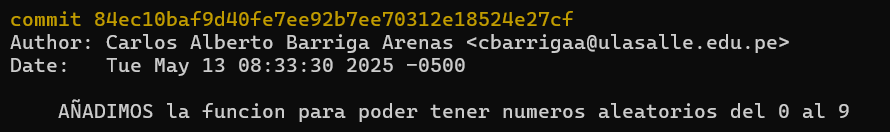
\includegraphics[width=1\textwidth]{img/commit_1.png}
  	\begin{lstlisting}[language=bash,caption={Actualisamos matrices-secuencial.cpp }][H]
		$ notepad matrices-secuencial.cpp
		$ git add matrices-secuencial.cpp
		$ git commit -m "ANADIMOS la funcion para poder tener numeros aleatorios del 0 al 9"
		$ git push -u origin main
	\end{lstlisting}
  	\begin{lstlisting}
        generarAleatorios();
        }
    void generarAleatorios() {
        for (int i = 0; i < size; ++i)
            for (int j = 0; j < size; ++j)
                datos[i][j] = rand() % 10; // Numeros randoms o aleatorios de 0 a 9
    }
	\end{lstlisting}
	\begin{itemize}	
		\item El commit seria : a4ae5b85ecb99aff0f7de4617d69bdae7aad8b0e
	\end{itemize}	
	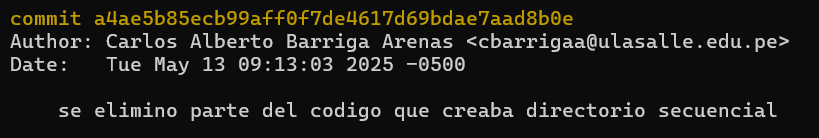
\includegraphics[width=1\textwidth]{img/commit_2.png}
	\begin{itemize}	
		\item Este seria el codigo final
	\end{itemize}

  	\begin{lstlisting}
#include <ctime>
#include <chrono>
#include <fstream>
#include <direct.h>  // Para crear directorios

using namespace std;
using namespace chrono;
@@ -22,7 +21,7 @@
    void generarAleatorios() {
        for (int i = 0; i < size; ++i)
            for (int j = 0; j < size; ++j)
                datos[i][j] = rand() % 10; // Numeros aleatorios de 0 a 9
                datos[i][j] = rand() % 10; // Números aleatorios de 0 a 9
    }

    int sumarElementos() {
@@ -34,44 +33,34 @@
    }
};

bool crearDirectorio(const string& path) {
    return _mkdir(path.c_str()) == 0;
}

int main() {
    srand(time(0)); // Semilla para números aleatorios
    int N;
    cout << "Ingrese el tamano maximo N de la matriz cuadrada: ";
    cin >> N;

    // Asegúrate de que la carpeta 'secuencial' exista
    if (!crearDirectorio("secuencial")) {
        cerr << "No se pudo crear el directorio 'secuencial'.\n";
        return 1;
    }

    ofstream archivo("secuencial/secuencial.csv");
    ofstream archivo("secuencial.csv");
    if (!archivo.is_open()) {
        cerr << "No se pudo abrir secuencial.csv para escritura.\n";
        return 1;
    }

    // Escribe los encabezados en el archivo CSV
    archivo << "Tamano de matriz,Tiempo de ejecucion (ms)\n";

    for (int n = 1; n <= N; ++n) {
        auto inicio = high_resolution_clock::now();
        Matriz matriz(n);
        int suma = matriz.sumarElementos();
        auto fin = high_resolution_clock::now();

        duration<double, milli> duracion = fin - inicio;

        archivo << n << "," << duracion.count() << endl;
        cout << "Matriz " << n << "x" << n << ": suma = " << suma
              << ", tiempo = " << duracion.count() << " ms\n";
    }

    archivo.close();
    return 0;
}
	\end{lstlisting}
        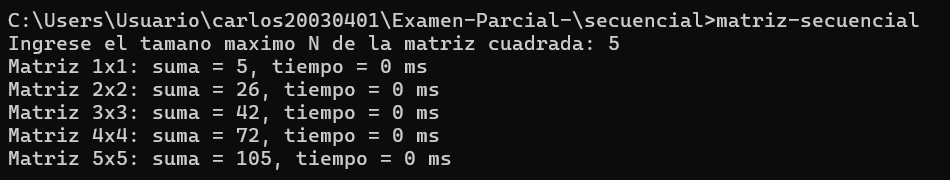
\includegraphics[width=1\textwidth]{img/resultado_1.png}        
	\subsection{Pseudocodigo}
        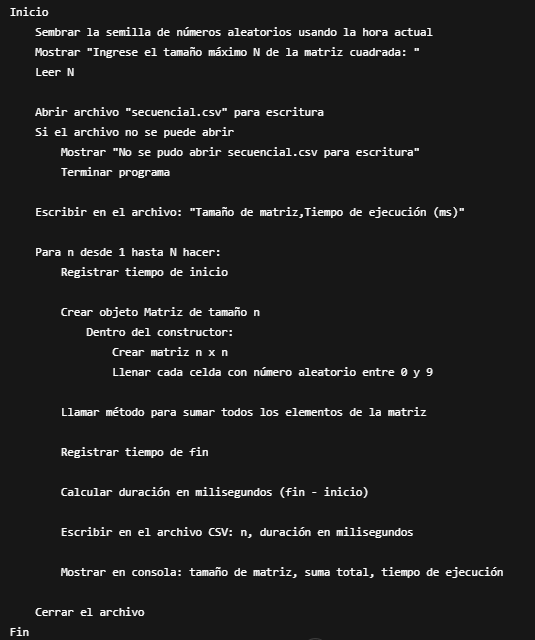
\includegraphics[width=1\textwidth]{img/pseudocodigo_1.png}        
	\begin{itemize}	
		\item Al graficarlo
	\end{itemize}
        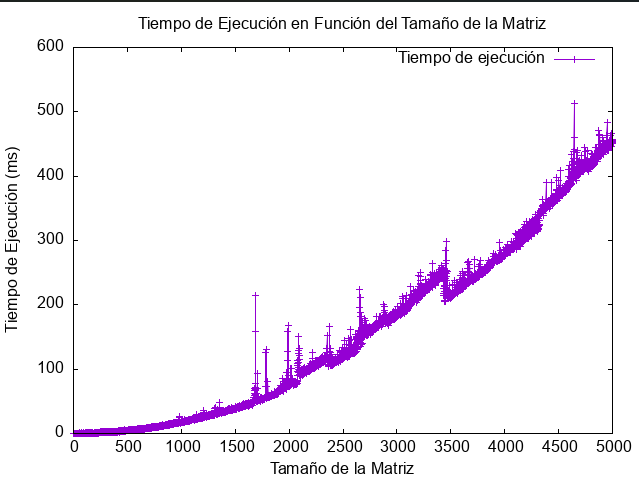
\includegraphics[width=1\textwidth]{img/grafica_1.png}










	
	\subsection{Matrices-Threads}
	\begin{itemize}	
		\item Creamos matrices-threads.cpp\end{itemize}	
		
	\begin{lstlisting}[language=bash,caption={Creamos en threads }][H]
		$ notepad matrices-threads.cpp
		$ git add matrices-threads.cpp
		$ git commit -m " creamos lo que es en threads el .cpp"
		$ git push -u origin main
	\end{lstlisting}
        \begin{lstlisting}
#include <iostream>
#include <vector>
#include <thread>
#include <chrono>
#include <random>


using namespace std;
mutex mtx;  // para proteger el acceso a la suma global

class Matriz {
private:
    int N;
    vector<vector<int>> datos;
public:
    Matriz(int n) : N(n), datos(n, vector<int>(n)) {
        random_device rd;
        mt19937 gen(rd());
        uniform_int_distribution<> dis(0, 9);
        for (int i = 0; i < N; ++i)
            for (int j = 0; j < N; ++j)
                datos[i][j] = dis(gen);
    }
    }
    int getValor(int i, int j) const {
        return datos[i][j]
    
	\end{lstlisting}
	\begin{itemize}	
		\item El commit seria :5eef6f197e4847fc6e0745b57c1a57a6bf747bb0
	\end{itemize}	

	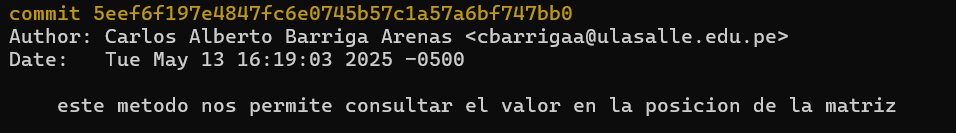
\includegraphics[width=1\textwidth]{img/commit_3.png}


  	\begin{lstlisting}[language=bash,caption={Actualisamos matrices-threads.cpp }][H]
		$ notepad matrices-threads.cpp
		$ git add matrices-threads.cpp
		$ git commit -m " este metodo nos permite consultar el valor en la posicion de la matriz"
		$ git push -u origin main
	\end{lstlisting}
  	\begin{lstlisting}
#include <iostream>
#include <vector>
#include <thread>
#include <chrono>
#include <random>

class Matriz {
private:
    int N;
    vector<vector<int>> datos;
public:
    Matriz(int n) : N(n), datos(n, vector<int>(n)) {
        random_device rd;
        mt19937 gen(rd());
        uniform_int_distribution<> dis(0, 9);
        for (int i = 0; i < N; ++i)
            for (int j = 0; j < N; ++j)
                datos[i][j] = dis(gen);
    }

    int getValor(int i, int j) const {
        return datos[i][j];
    }

    int getSize() const {
        return N;
    }
};
void sumarFila(const Matriz& matriz, int filaInicio, int filaFin, long long& sumaParcial) {
    long long localSuma = 0;
    for (int i = filaInicio; i < filaFin; ++i) {
        for (int j = 0; j < matriz.getSize(); ++j) {
            localSuma += matriz.getValor(i, j);
        }
    }
    lock_guard<mutex> lock(mtx);
    sumaParcial += localSuma;
}

int main() {
    int N;
    cout << "Ingrese el valor de N: ";
    cin >> N;
    ofstream archivo("threads.csv");
    archivo << "Tamaño de matriz,Tiempo de ejecución (ms)\n";


    for (int n = 1; n <= N; ++n) {
        Matriz matriz(n);
        long long sumaTotal = 0;
        int numThreads = thread::hardware_concurrency();
        vector<thread> threads
        int filasPorHilo =  / numThreads;
        int resto = n % numThreads;
        auto inicio = chrono::high_resolution_clock::now();
        auto inicio = chrono::high_resolution_clock::now();
        int inicioFila = 0;
        for (int i = 0; i < numThreads; ++i) {
            int finFila = inicioFila + filasPorHilo + (i < resto ? 1 : 0);
            threads.emplace_back(sumarFila, ref(matriz), inicioFila, finFila, ref(sumaTotal));
            inicioFila = finFila;
        }
	\end{lstlisting}
	\begin{itemize}	
		\item El commit seria : de8fd54c03b94a8b718b6962999239a842d3a4e0
	\end{itemize}	
 
	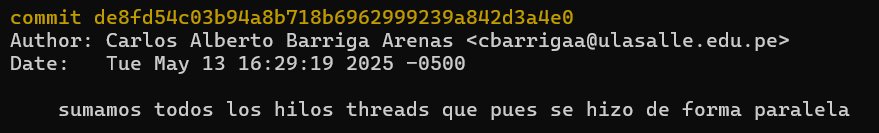
\includegraphics[width=1\textwidth]{img/commit_4.png}


	\begin{itemize}	
		\item Este seria el codigo final

	\end{itemize}


 
  	\begin{lstlisting}
#include <iostream>
#include <vector>
#include <thread>
#include <chrono>
#include <fstream>
#include <mutex>
#include <random>

using namespace std;
mutex mtx;  // para proteger el acceso a la suma global

class Matriz {
private:
    int N;
    vector<vector<int>> datos;
public:
    Matriz(int n) : N(n), datos(n, vector<int>(n)) {
        random_device rd;
        mt19937 gen(rd());
        uniform_int_distribution<> dis(0, 9);
        for (int i = 0; i < N; ++i)
            for (int j = 0; j < N; ++j)
                datos[i][j] = dis(gen);
    }

    int getValor(int i, int j) const {
        return datos[i][j];
    }

    int getSize() const {
        return N;
    }
};

void sumarFila(const Matriz& matriz, int filaInicio, int filaFin, long long& sumaParcial) {
    long long localSuma = 0;
    for (int i = filaInicio; i < filaFin; ++i) {
        for (int j = 0; j < matriz.getSize(); ++j) {
            localSuma += matriz.getValor(i, j);
        }
    }
    lock_guard<mutex> lock(mtx);
    sumaParcial += localSuma;
}

int main() {
    int N;
    cout << "Ingrese el tamano maximo N de la matriz cuadrada: ";
    cin >> N;

    ofstream archivo("threads.csv");
    archivo << "Tamaño de matriz,Tiempo de ejecución (ms),Suma total\n";

    for (int n = 1; n <= N; ++n) {
        Matriz matriz(n);
        long long sumaTotal = 0;

        int numThreads = thread::hardware_concurrency();
        numThreads = numThreads > n ? n : numThreads;
        numThreads = numThreads > 0 ? numThreads : 4;

        vector<thread> threads;
        int filasPorHilo = n / numThreads;
        int resto = n % numThreads;

        auto inicio = chrono::high_resolution_clock::now();

        int inicioFila = 0;
        for (int i = 0; i < numThreads; ++i) {
            int finFila = inicioFila + filasPorHilo + (i < resto ? 1 : 0);
            threads.emplace_back(sumarFila, ref(matriz), inicioFila, finFila, ref(sumaTotal));
            inicioFila = finFila;
        }

        for (auto& t : threads) {
            t.join();
        }

        auto fin = chrono::high_resolution_clock::now();
        chrono::duration<double, milli> duracion = fin - inicio;

        archivo << n << "," << duracion.count() << "," << sumaTotal << "\n";
        cout << "Matriz " << n << "x" << n << ": suma = " << sumaTotal
             << ", tiempo = " << static_cast<int>(duracion.count()) << " ms" << endl;
    }

    archivo.close();
    return 0;
}

	\end{lstlisting}



 
        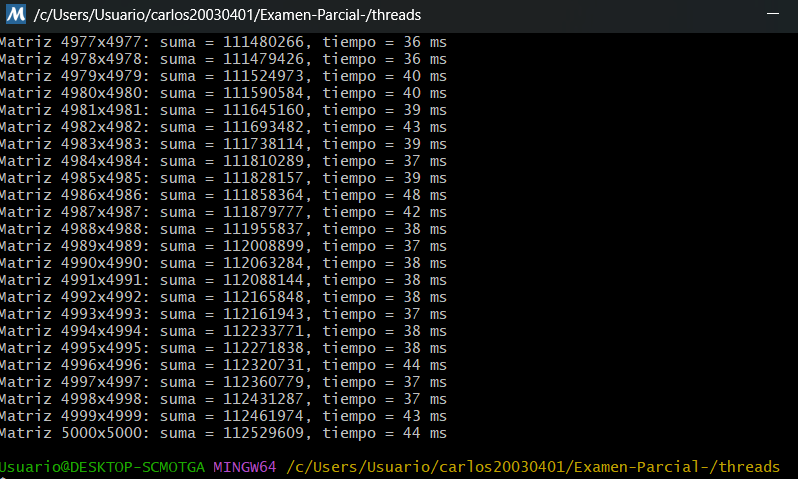
\includegraphics[width=1\textwidth]{img/resultado_2.png}


	\begin{itemize}	
		\item Aca cabe aclarar que se uso Msys2 por problemas de versiones en cmd y g++

	\end{itemize}

        
        
	\subsection{Pseudocodigo}



        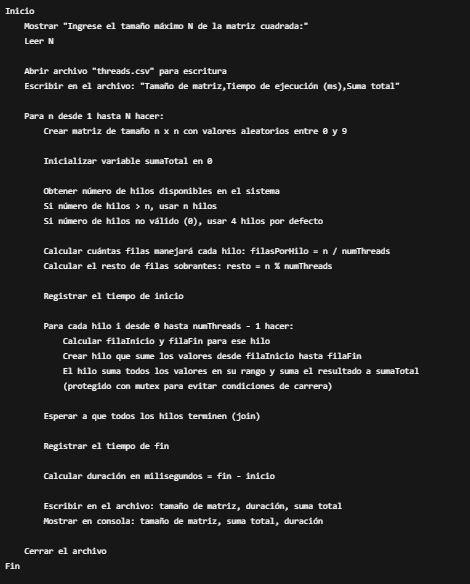
\includegraphics[width=1\textwidth]{img/pseudocodigo_2.png}
        
	\begin{itemize}	
		\item Al graficarlo
	\end{itemize}


        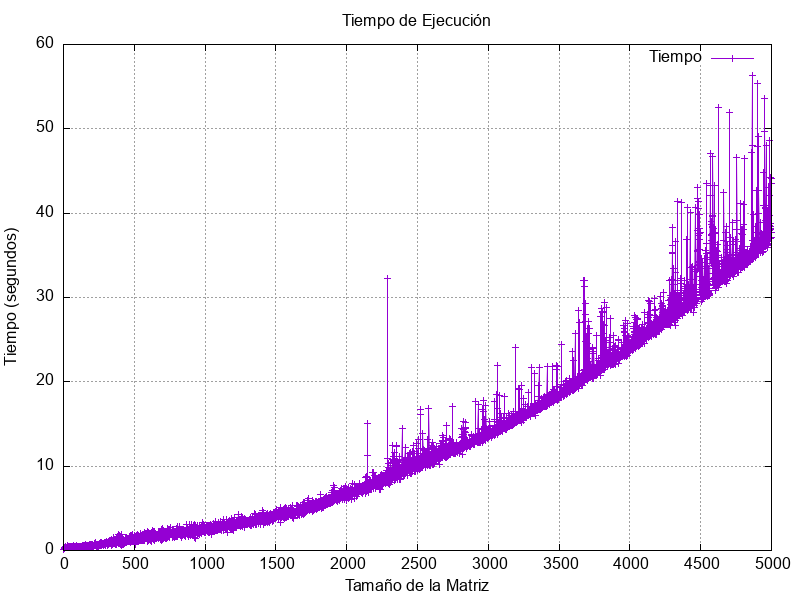
\includegraphics[width=1\textwidth]{img/grafica_2.png}


	\begin{itemize}	
		\item Se probo con 5000 matrices demoro aprox. unos 15 min

	\end{itemize}






		

\section{\textcolor{red}{Calificación}}

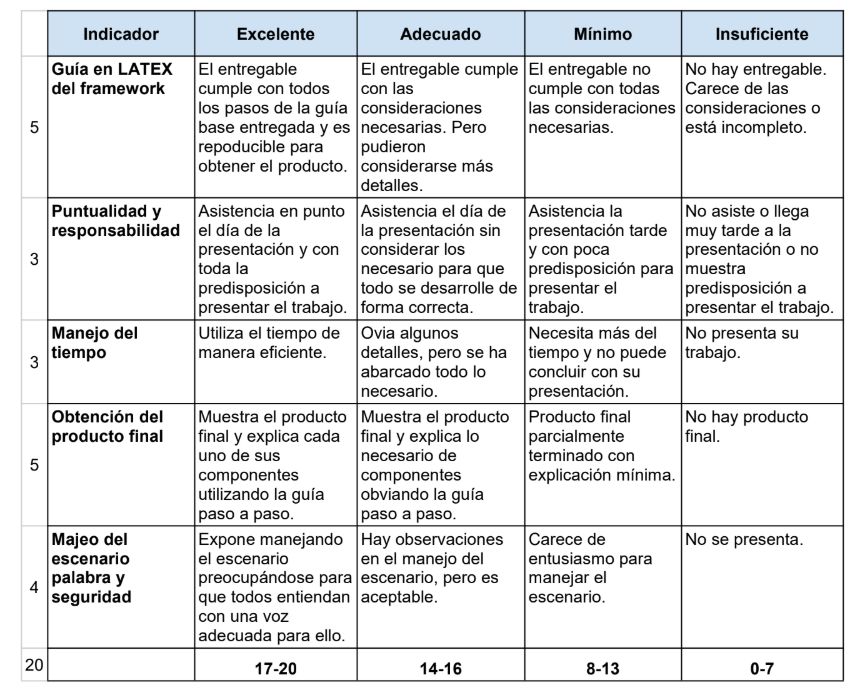
\includegraphics[width=1\textwidth]{img/calificacion.png}

	
\clearpage

\section{Referencias}
\begin{itemize}			
	\item \url{https://github.com/}
	\item \url{https://www.onlinegdb.com/fork/trSsLe7w1}
 	\item \url{https://www.msys2.org/#sponsors}
  	\item \url{https://www.mingw-w64.org/downloads/}
   	\item \url{https://azulschool.net/todos-los-grupos/grupo-de-c/forum/topic/generar-numeros-aleatorios-en-c/}
	\item \url{https://www.w3resource.com/cpp-exercises/vector/cpp-vector-exercise-3.php}



    
\end{itemize}	
	
%\clearpage
%\bibliographystyle{apalike}
%\bibliographystyle{IEEEtranN}
%\bibliography{bibliography}
\end{document}